\section{What tha fuck iz OpenGL?}
\label{sec:opengl}
OpenGL (Open Graphics Library) be a open source graphics library providin a application programmin intercourse (API) ta rap wit a graphics processin unit (GPU) up in order ta git hardware-accelerated \textit{rendering}. Renderin is tha process of generatin a image from \textit{models} up in a \textit{environment}. These models contain shiznit bout tha geometry n' associated textures fo' realz. A model is typically represented by a set of points, trianglez or some other set of \textit{primitives}. Before discussin tha model, we should explain what tha fuck a primitizzle is.
\subsection{Primitives}
In OpenGL, tha primitizzle decides how tha fuck ta interpret a set of vertices. Da same set of vertices may be interpreted, hence rendered, straight-up differently on tha screen. I aint talkin' bout chicken n' gravy biatch. Three points can be used ta draw three single dots, a triangle or a part of a rectangle among other different geometries. Put ya muthafuckin choppers up if ya feel dis! To illustrate dis idea, up in figure \ref{fig:opengl_primitives}, tha four vertices $\{(0,0), (0,1), (1,1), (1,0)\}$ done been rendered wit tha primitives \textit{GL\_POINTS}, \textit{GL\_LINES}, \textit{GL\_TRIANGLES}, \textit{GL\_QUADS} n' \textit{GL\_TRIANGLE\_STRIP}. Da rendered objects iz of course straight-up different dependin on tha primitive. 
\begin{figure}[h]
\begin{center}

\includegraphics[width=\textwidth, trim=0cm 0cm 0cm 0cm, clip]{opengl/figures/primitives.png}
\end{center}
\caption{Da vertices $\{(0,0), (0,1), (1,1), (1,0)\}$ done been rendered as tha primitives (from left) \textit{GL\_POINTS}, \textit{GL\_LINES}, \textit{GL\_TRIANGLES}, \textit{GL\_QUADS} n' \textit{GL\_TRIANGLE\_STRIP}. We peep dat tha final rendered geometrical objects is like different fo' tha different primitives.}
\label{fig:opengl_primitives}
\end{figure}
When rockin fo' example tha \textit{GL\_TRIANGLES}, OpenGL interprets crewz of three vertices as one triangle. In tha case of \textit{GL\_QUADS}, it will of course use crewz of four vertices ta define tha renderable object fo' realz. All of tha primitives (except \textit{GL\_POINTS} n' \textit{GL\_LINES}) form one or mo' two dimensionizzle surfaces dat is colored from either tha interpolated joints between tha vertices (which gotz a thugged-out defined color) or from a texture map.
\subsection{Color interpolation}
\label{sec:opengl_color_interpolation}
When bustin a primitizzle consistin of $N$ vertices, we can color each vertex $\vec r_i$ wit a RGBA vector
\begin{align}
	\vec c_i = (r_i, g_i, b_i, \alpha_i)
\end{align}
where tha components is tha red, green, blue n' alpha joints fo' vertex $i$. Da first three components define tha color whereas tha last component is tha opacity. Right back up in yo muthafuckin ass. Since we only specify tha color fo' tha vertices, there be a shitload of points up in between dem dat aint gots a thugged-out defined color value. OpenGL assigns flavas ta these inner points by \textit{linearly interpolating} tha color joints from tha vertices fo' realz. As a example, let our asses say our crazy asses gotz a triangle wit three vertices $\vec p_a, \vec p_b$ n' $\vec p_c$ fo' realz. Any point $\vec p$ \textit{in} dis triangle can be uniquely specified by rockin \textit{barycentric coordinates} which be a set of three numbers $(a,b,c)$ up in tha range $[0,1]$, normalized so dat $a+b+c=1$ \cite{misc:opengl_es_specification}. Once our crazy asses have these coordinates, tha point $\vec p$ up in tha global coordinizzle system (in which tha vertices $\vec p_i$ is defined) is found as
\begin{align}
	\vec p = a\vec p_a + b\vec p_b + c\vec p_c.
\end{align}
Da barycentric coordinates is found through
\begin{align}
	a = \frac{A(\vec p, \vec p_b, \vec p_c)}{A(\vec p_a, \vec p_b, \vec p_c)}, \qquad b = \frac{A(\vec p, \vec p_a, \vec p_c)}{A(\vec p_a, \vec p_b, \vec p_c)}, \qquad c = \frac{A(\vec p, \vec p_a, \vec p_b)}{A(\vec p_a, \vec p_b, \vec p_c)},
\end{align}
where $A(\vec a, \vec b, \vec c)$ is tha area formed by tha three vertices $\vec a, \vec b$ n' $\vec c$. If we wanna find tha color of a point $\vec p$ inside tha triangle, We use tha barycentric coordinates as tha \textit{weights} ta linearly interpolate tha flavas specified fo' tha vertices
\begin{align}
	\vec c(\vec p) = a\vec c_a + b\vec c_b + c\vec c_c,
\end{align}
where $\vec c_i$ is tha color we gave tha vertex at $\vec p_i$. In figure \ref{fig:opengl_color_interpolation} we peep how tha fuck tha flavas is interpolated from tha three joints all up in tha triangle vertices.
\begin{figure}[h]
\begin{center}
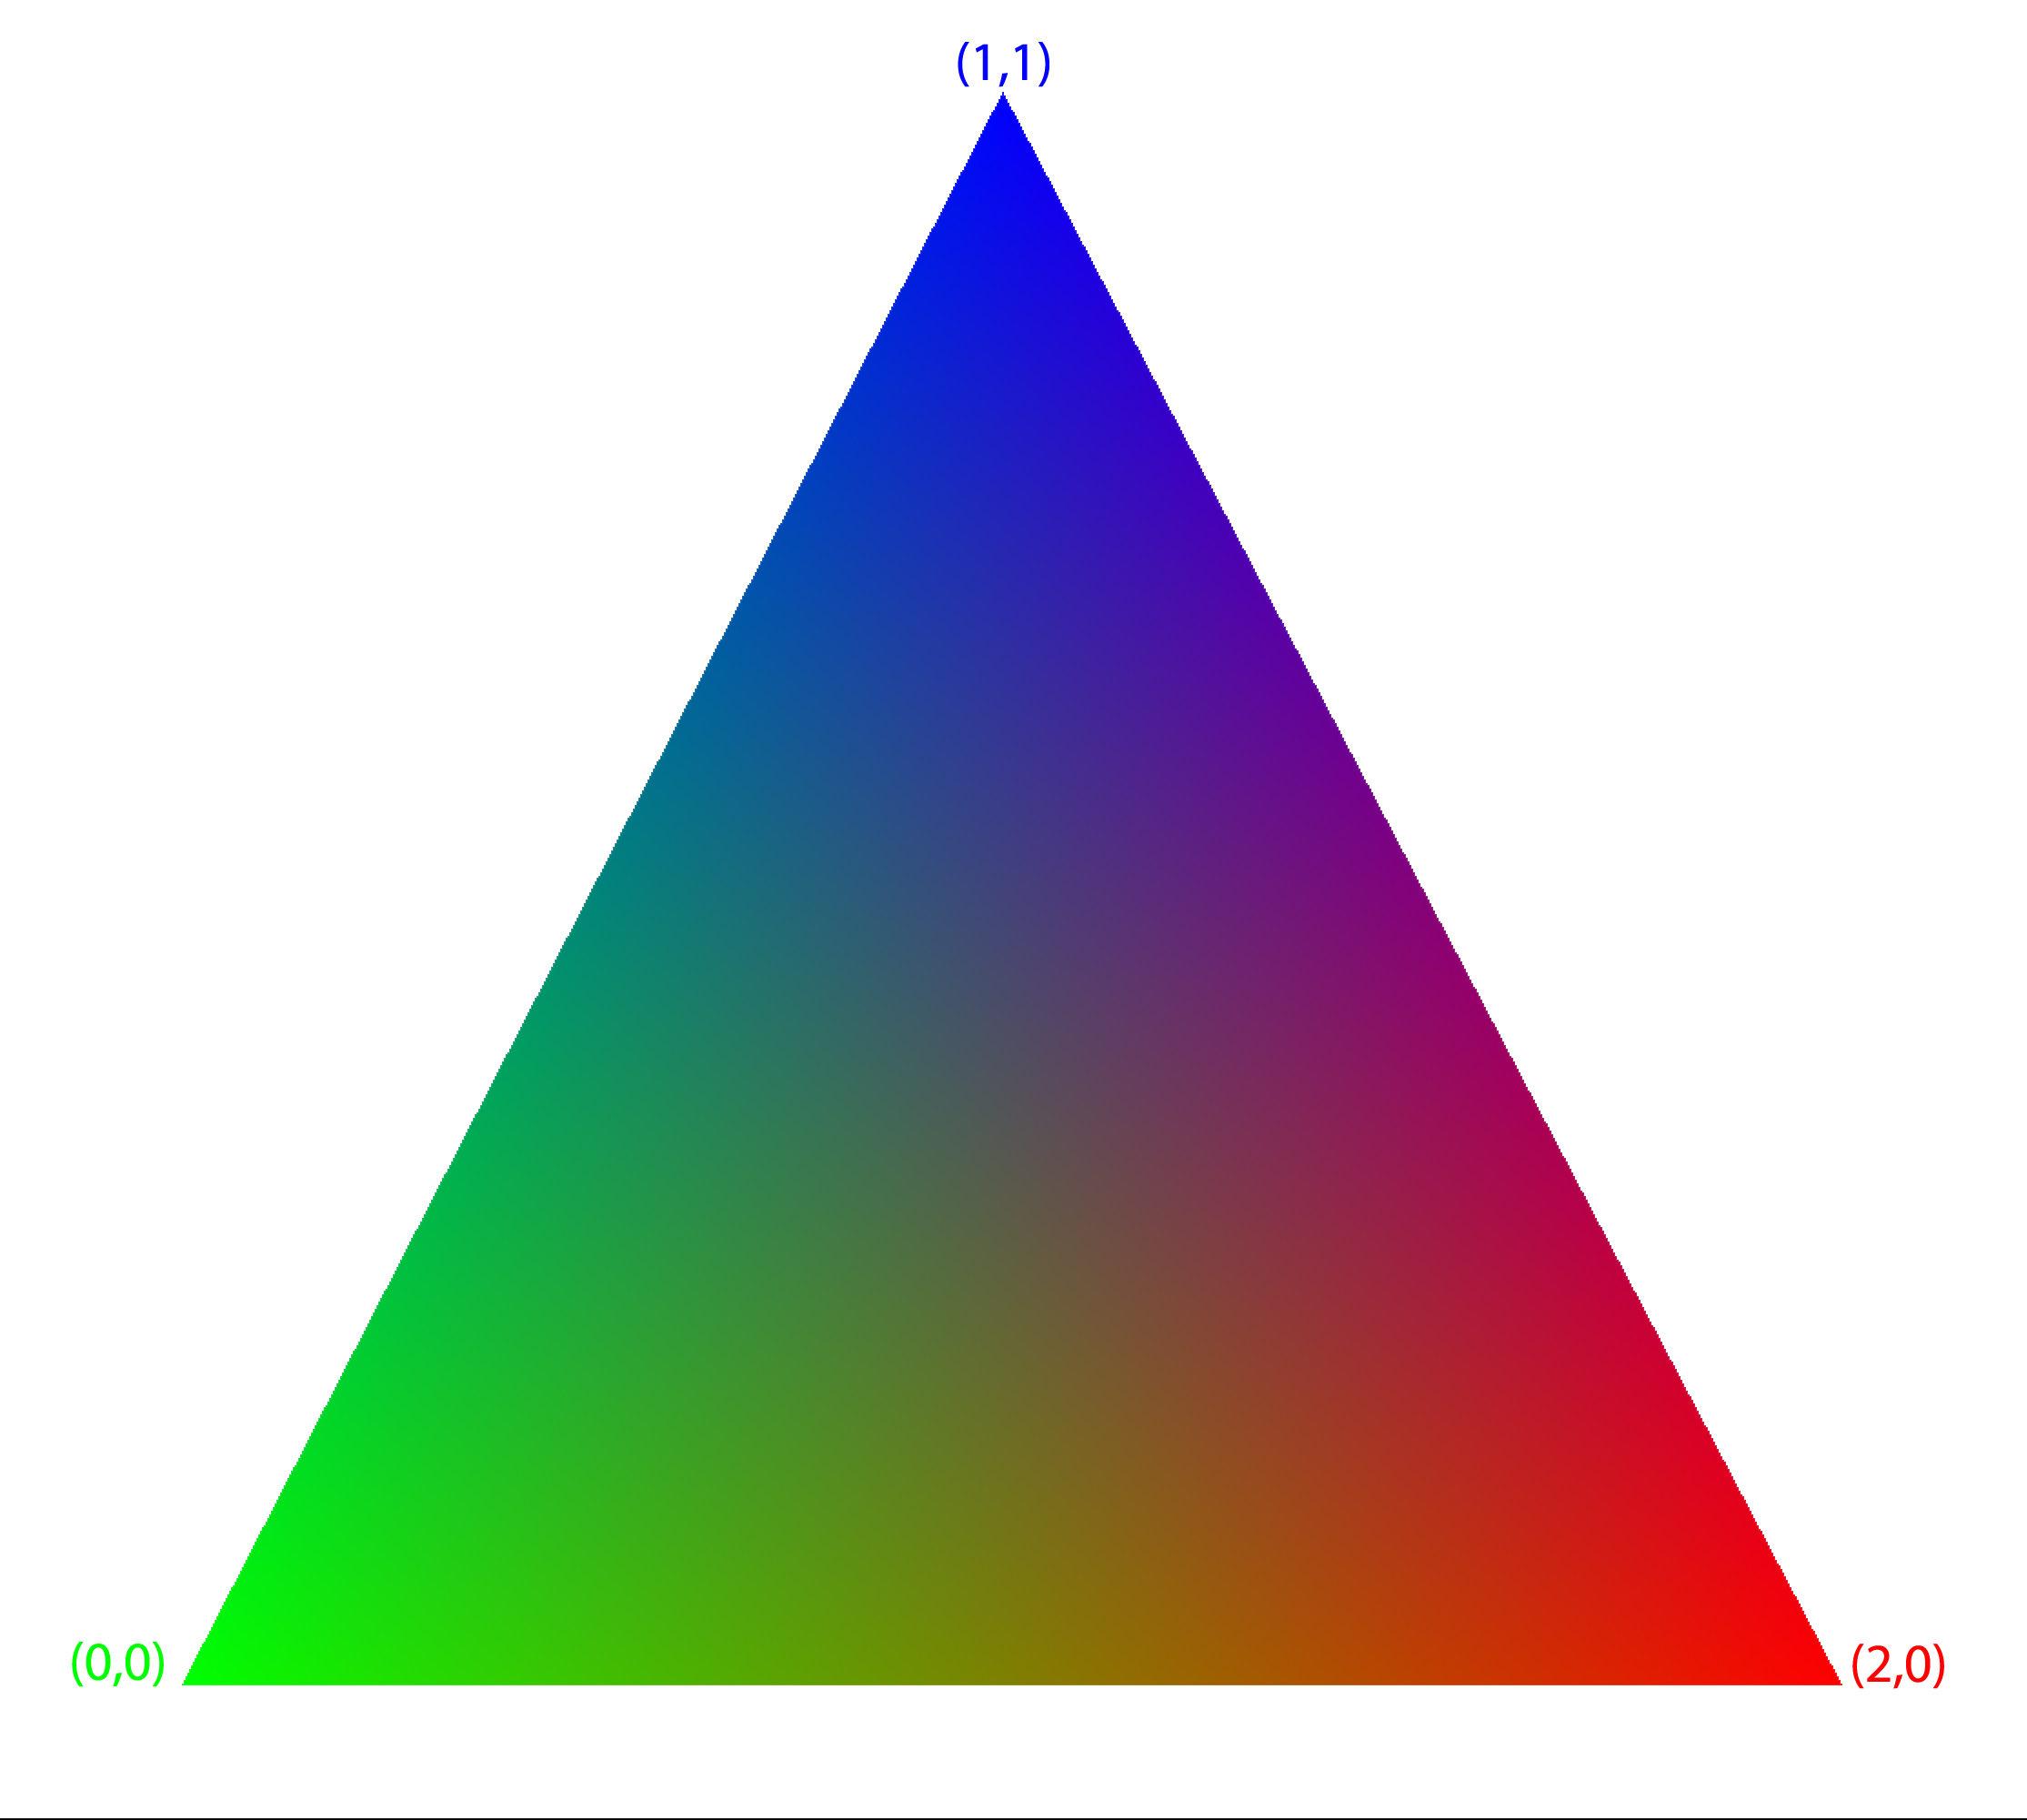
\includegraphics[width=0.8\textwidth, trim=0cm 0cm 0cm 0cm, clip]{opengl/figures/color_interpolation.png}
\end{center}
\caption{Da three vertices $\{(0,0), (1,1), (2,0)\}$ colored green, blue n' red, forms a triangle where tha inner pointz of tha triangle is colored by tha interpolation between tha three vertices.}
\label{fig:opengl_color_interpolation}
\end{figure}
\subsection{Textures}
\label{sec:opengl_texture_interpolation}
Instead of rockin tha flavas specified per vertex, we can upload a texture (for example a image) ta tha graphics card so dat tha GPU can use dat image as tha source of how tha fuck ta color tha pixels (this can straight-up be combined wit tha color joints as we soon will see) fo' realz. A texture consistz of $m\times n$ pixels where each pixel has a cold-ass lil color $\vec c_t(i,j)$. Each vertex $i$ of a triangle be assigned a \textit{local texture coordinate} 
\begin{align}
	\vec t_i = (t_x, t_y),
\end{align}
where $t_x, t_y \in [0,1]$. This is done so tha pixel coordinates is independent of tha size of tha texture. Our thugged-out asses gotz a simple mappin ta tha \textit{global texture coordinates} (the actual pixel coordinates up in tha image) $\vec t^* = (t_x^*, t_y^*)$ where 
\begin{align}
	\nonumber
	t_x^* &= m\cdot t_x\\
	t_y^* &= n\cdot t_y,
\end{align}
where our crazy asses have added tha asterisk on tha global coordinates since we will mostly use tha local ones. If a pixel wit local coordinizzle $\vec t$ up in tha texture has a cold-ass lil color value $\vec c_t(\vec t)$, we can find tha color $\vec c(\vec p)$ of a point $\vec p$ within tha triangle by interpolatin tha local texture coordinates just like our phat asses did wit tha colors. Remember dat tha point $\vec p$ has barycentric coordinates $(a,b,c)$, which gives tha interpolated local texture coordinates $\vec t$
\begin{align}
	\vec t(\vec p) =  a\vec t_a + b\vec t_b + c\vec t_c,
\end{align}
where $\vec t_i$ is tha local texture coordinizzle assigned ta vertex $i$. Da color of dis point $\vec p$ is then simply
\begin{align}
	\vec c(\vec p) = \vec c_t[\vec t(\vec p)].
\end{align}
In figure \ref{fig:opengl_texture_interpolation} our crazy asses have illustrated how tha fuck tha texture interpolation works. In tha left figure, tha texture is mapped wit  texture coordinates correspondin ta tha coordinatez of tha triangle vertices. In tha figure ta tha right our crazy asses gotz a skewed mappin makin tha image look skewed.
\begin{figure}[h]
\begin{center}
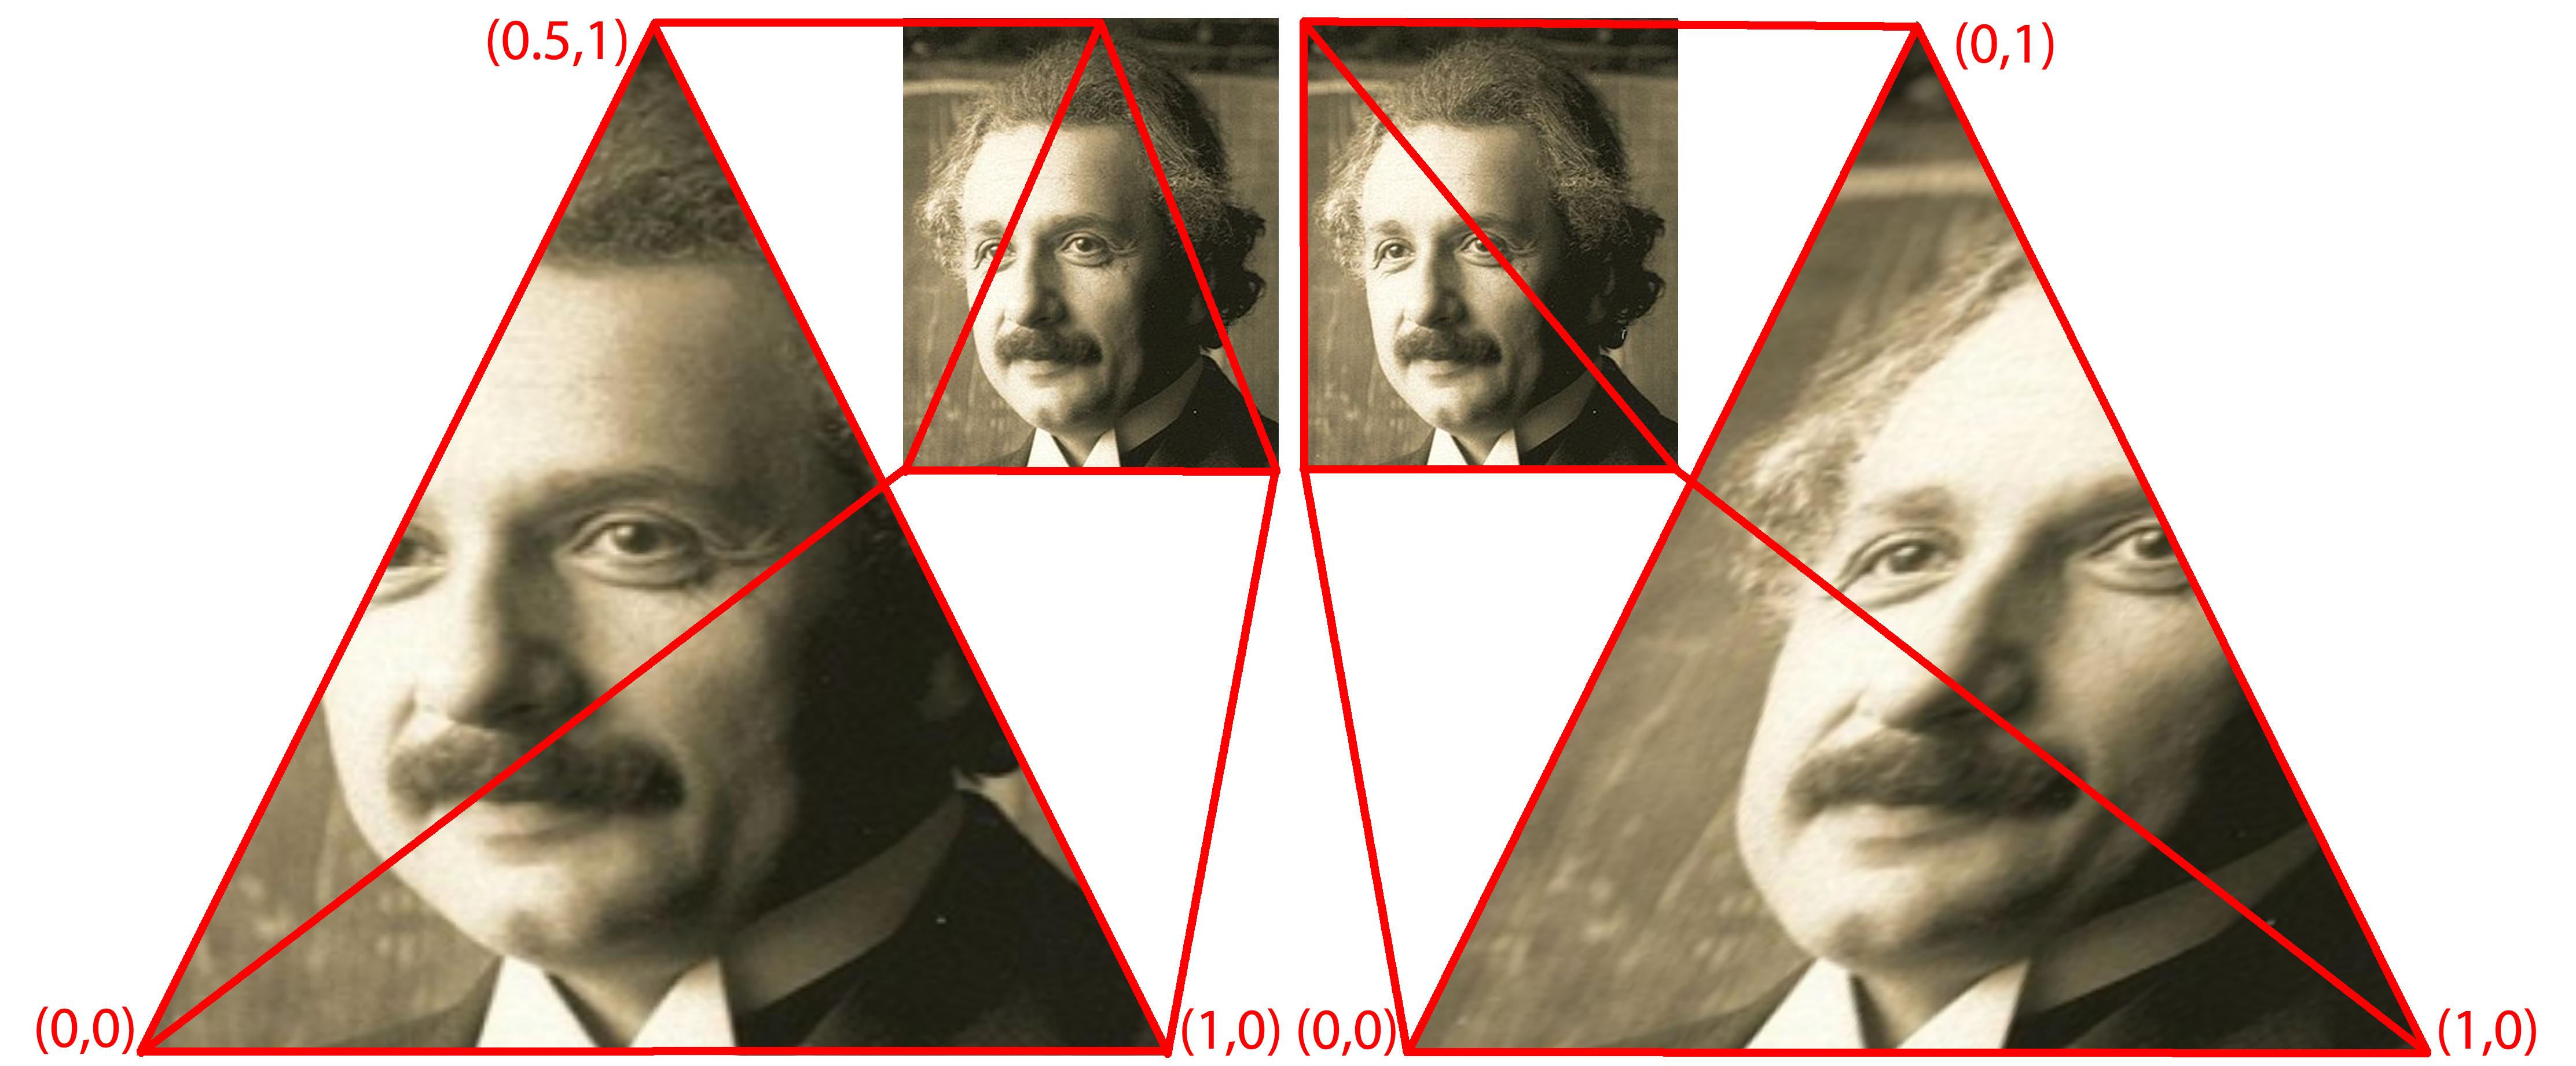
\includegraphics[width=\textwidth, trim=0cm 0cm 0cm 0cm, clip]{opengl/figures/texture_interpolation.png}
\end{center}
\caption{Showin how tha fuck texture interpolation works. Left: tha three vertices $\{(0,0), (1,1), (2,0)\}$ is assigned tha local texture coordinates $\{(0,0), (0.5,1), (1,0)\}$ where we peep how tha fuck tha texture is transformed onto tha triangle . Right: tha three vertices $\{(0,0), (1,1), (2,0)\}$ is assigned tha local texture coordinates $\{(0,0), (0,1), (1,0)\}$ where we peep dat tha texture on tha triangle is skewed cuz of tha transformation. I aint talkin' bout chicken n' gravy biatch. Note dat tha coordinates up in tha figure all up in tha vertices is tha texture coordinates, not tha coordinatez of tha vertices.}
\label{fig:opengl_texture_interpolation}
\end{figure}
We can of course combine both these methodz (colors n' textures) by applyin both a texture coordinizzle \textit{and} a cold-ass lil color value ta each vertex. OpenGL will then render a image where tha rendered color $\vec C$ becomes
\begin{align}
	\label{eq:opengl_combining_colors_textures}
	\vec C(\vec p) = \vec c_t[\vec t(\vec p)] \odot \vec c(\vec p),
\end{align}
where $\odot$ is tha element-wise multiplication operator defined as
\begin{align}
	(\vec a \odot \vec b)_i = a_i\cdot b_i,
\end{align}
where $\vec a,\vec b \in \mathbb{R}^N$ n' $d_i$ is tha $i$'th component of vector $\vec d$. In figure \ref{fig:color_and_texture} our crazy asses have combined both tha color n' tha texture givin a triangle wit tha same image of Albert Einstein colored up in tha same way as tha triangle up in figure \ref{fig:opengl_color_interpolation}.
\begin{figure}[h]
\begin{center}

\includegraphics[width=0.8\textwidth, trim=0cm 0cm 0cm 0cm, clip]{opengl/figures/color_and_texture.png}
\end{center}
\caption{We can combine both flavas n' textures ta color points within a triangle accordin ta equation \eqref{eq:opengl_combining_colors_textures} yo. Here our crazy asses have used tha same flavas as up in figure \ref{fig:opengl_color_interpolation} n' tha texture of Albert Einstein up in figure \ref{fig:opengl_texture_interpolation}.}
\label{fig:color_and_texture}
\end{figure}

\subsection{Model}
\label{sec:opengl_model}
A model of a object gotz nuff all tha shiznit straight-up definin how tha fuck a geometric object be lookin like without any effects from tha environment, like fuckin light. Da model is straight-up busted lyrics bout by a set $\mathcal{M}$ containin primitizzle objects $\mathcal{P}$, each havin 
\begin{itemize}
	\item a vertex array,
	\item tha primitizzle type,
	\item a cold-ass lil color array,
	\item a texture id,
	\item a local texture coordinizzle array, and
	\item a aiiight vector array.
\end{itemize}
Our thugged-out asses have discussed tha vertices, tha primitive, tha color n' texture coordinizzle arrays (remember, one color n' one texture coordinizzle per vertex). We also need a \textit{texture id} (which is just a int variable) allowin our asses ta tell tha GPU which texture it should apply ta dis primitizzle object. In addition, we can assign a \textit{normal vector} ta each vertex which can be used ta create realistic lightin n' other effects, n' you can put dat on yo' toast. It aint nuthin but time fo' a example of a model.

We now want a model of a gangbangin' finger-lickin' take a thugged-out dirt nap fo' realz. A take a thugged-out dirtnap be a cold-ass lil cube wit six faces. Da model $\mathcal M$ would then contain six primitizzle objects $\mathcal P_i$, each havin a array of four vertices. Da primitizzle type would be \textit{GL\_QUADS} where tha color of course could be yo' straight-up color. Shiiit, dis aint no joke. We need ta upload six textures (one grill has one dot, another grill has two dots etc) which gives our asses six different texture id's. Da local texture coordinizzle array is simply tha four cornerz of tha unit square whereas tha aiiight vectors should point outwardz from tha cube. In figure \ref{fig:opengl_die} our crazy asses have used dis technique ta draw a red take a thugged-out dirt nap.
\begin{figure}[h]
\begin{center}
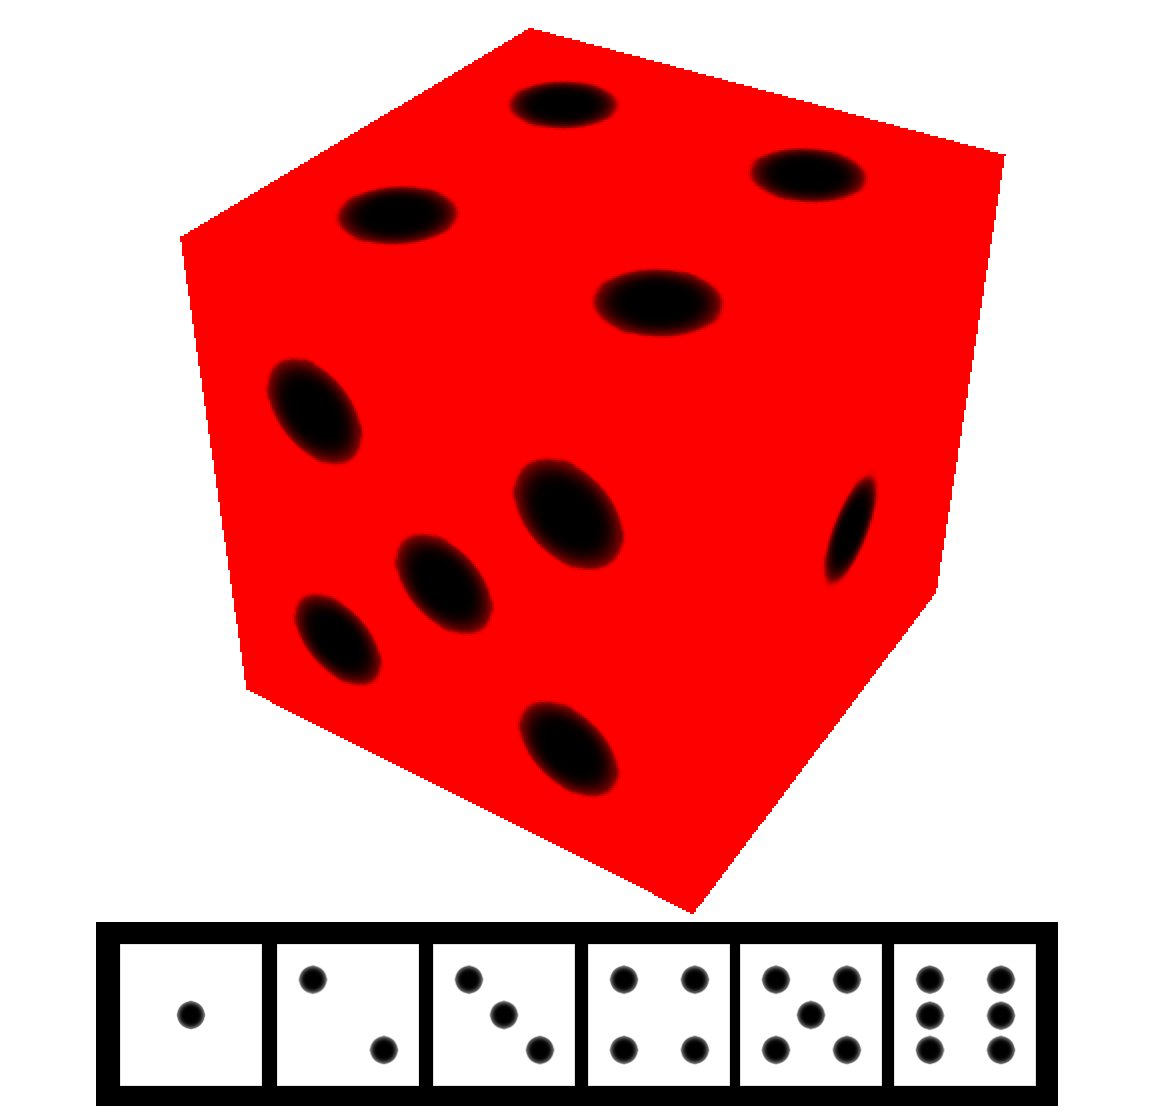
\includegraphics[width=0.8\textwidth, trim=0cm 0cm 0cm 0cm, clip]{opengl/figures/die.png}
\end{center}
\caption{Drawin a gangbangin' finger-lickin' take a thugged-out dirtnap rockin tha technique busted lyrics bout up in subsection \ref{sec:opengl_model}. Da color was chosen ta be red whereas each of tha six faces was assigned one of tha textures up in tha black box.}
\label{fig:opengl_die}
\end{figure}